\documentclass[12pt]{article}
\usepackage{float}
\usepackage{graphicx}
\usepackage{amsmath}
\usepackage{tikz}
\usepackage[ruled,linesnumbered,noend]{algorithm2e}
\usepackage{caption}
\usepackage{wrapfig}
\usepackage{geometry}
\geometry{a4paper,scale=0.75}
\usepackage{subfigure}
\usepackage{titlesec}
\usepackage{fancyhdr}
\titleformat{\section}
  {\normalfont\huge\bfseries}{\thesection}{1em}{}
\captionsetup[algorithm2e]{labelsep=colon}

\pagestyle{fancy}
\fancyhf{}
\rhead{Online Property Sales}
\lhead{COMP9900 Project Proposal}

\begin{document}

\begin{titlepage}
  \centering
  {\centering
    
\includegraphics[height=0.3\textheight]{images/unsw.png}\par
  }
  \vspace{1cm}
  {\scshape\huge COMP9900 Project Proposal\par}
  \vspace{2cm}
  \large 21 Sep, 2020\\ 
  
  \begin{center}
    \renewcommand{\arraystretch}{1.5}
    \begin{tabular}{r l l} 
         Srcum master/Frontend& Wanchao\ Huang &z5192415\\
         Frontend             & Raymond\ Lu     &z5277884\\
         Backend              & Tao\ Xue       &z5219280\\
         Backend              & Xiaohan\ Zhu    &z5187021\\
         Frontend             & Ziqi\ Liang     &z5202297\\ 
    \end{tabular}\\
\end{center}
  \vspace{1cm}
\end{titlepage}

\tableofcontents
\newpage

\section{Background}
Ziqi
\subsection{Problem statement}
\subsection{Existing systems analysis}

\newpage
\section{User stories}
Raymond
\subsection{Product backlog of user stories}
\subsection{Product backlog in Jira}

\newpage
\section{Sprints}
Wanchao

\newpage
\section{Interface and Flow Diagram}
Wanchao

\newpage
\section{System Architecture}
\paragraph{}
\subsection{Separate Front-end and Back-end system}
\centerline{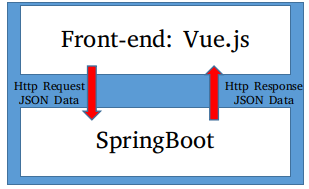
\includegraphics[scale = 0.5]{pic/g1.png}}

We choose to split the whole system into two subsystems: \textbf{Frontend System} which
is for presentation purpose and the \textbf{Backend System} to realize the requirement. Thus
the two subsystems are not dependent much on each other. So that, we can develope and test 
out codes independently and easily scale up and upgrade.
\subsection{Front-end}
We are using \textbf{Vue.js} framework for our front-end system. Comparing with traditional
\textit{HTML} and other static template, Vue framework can bring in dynamic and fancy effects. 
Comparing to other front-end frameworks such as Angular and React, 
Vue is much flatter learning curve and the higher coding speed.

\subsection{Back-end}
\centerline{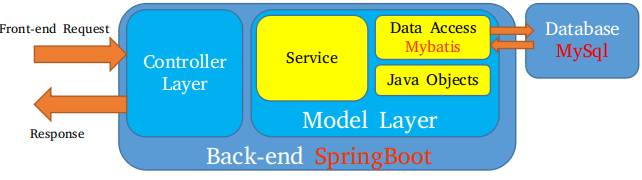
\includegraphics[scale = 0.5]{pic/g2.png}}
\subsubsection{Basic Framework}
The language we used is \textbf{Java} and  basic framework chosen to realize the overall architecture is \textbf{Spring Boot} 
which  embeds Tomcat server and 
gathers common java-web development frameworks. Thus, we can build up and deploy the
whole system easily.
\subsubsection{Back-end Architecture}
For decoupling, we adopt a MVC three-layer architecture: 
\begin{itemize}
  \item \textbf{Model Layer}: Data persistence and process  requests.
  \begin{itemize}
    \item Service Layer: Deal with specific business.
    \item Data Access Object: Communicate with database.
    \item Plain Java Objects
  \end{itemize}
  \item \textbf{View Layer}: Represent the data, in our architecture is replace by the front-end system.
  \item \textbf{Controller Layer}: Receive HTTP request based on the url from the Front-end and return results from the Model layer.
\end{itemize}

\subsubsection{Data Access}
\centerline{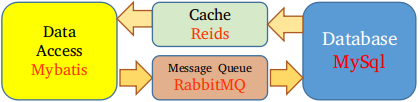
\includegraphics[scale = 0.5]{pic/g3.png}}
In model layer, we need to fetch and update data in database. To simplify programs and 
improve development efficiency, we are using an ORM framework Mybatis. Besides that

Then we want to reduce the pressure of database reading and writing. Thus, we 
introduce \textbf{Redis} as the cache of reading data, and a message queue \textbf{(RabbitMQ)}
to improve asynchronousity and concurrency.

\subsubsection{Authentication and Authorization}
\centerline{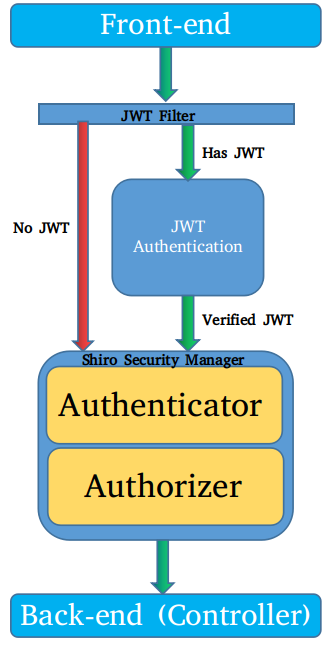
\includegraphics[scale = 0.44]{pic/g4.png}}
In our system, there are three roles: Anonymous, Users and Registered Auction Bidders (RAB). Thus, we
need a efficient and simple authentication and authorization framework. Thus we are using  a security framework called
\textbf{Shiro} along with \textbf{J}ason \textbf{W}eb \textbf{T}oken to achieve this need.

\subsection{Conclusion}
Our system architecture has:
\begin{itemize}
  \item A clear description showing the presentation, business and data layers in the system, and what each layer contains
  \item external actors and how they interact with system
\item clear description of the technologies/languages planned for use
\end{itemize}

And technologies in Use:
\begin{itemize}
  \item Front-end
  \begin{itemize}
    \item Vue.js
  \end{itemize}
\end{itemize}
\begin{itemize}
  \item Back-end
  \begin{itemize}
    \item Develop Language: Java
    \item  Framework: Spring Boot
    \item Database in USE: MySQL
    \item Persistence Layer: MyBatis
    \item Cache and NoSQL: Redis
    \item Message Queue: RabbitMQ
    \item Authentication and Authorization: Shiro + JWT
    \item Cloud: AWS
  \end{itemize}
\end{itemize}

\end{document}